Network Intrusion Detection Systems (NIDS) sind Anwendungen, die versuchen, schädliche Aktivitäten im Netzwerk zu erkennen, indem sie dessen gesamten Traffic aufzeichnen und analysieren. Ein beliebtes NIDS-Programm ist das free/open-source tool \textbf{snort}, welches hier zum Einsatz kommt. Es bietet ein modulares Konfigurationssystem über sog. \textit{rules} für Traffic- und Protokollanalysen sowie die Erkennung verschiedenster Angriffe über Signaturmatching.\\

Dieses Dokument beschreibt die Installation einer Testumgebung für snort auf Basis von VirtualBox, welche anschließend durch verschiedene Angriffe getestet wird. Die Netzwerkstruktur zeigt die folgende Abb. \ref{fig:network-structure}.

\begin{figure}[H]
  \centering
  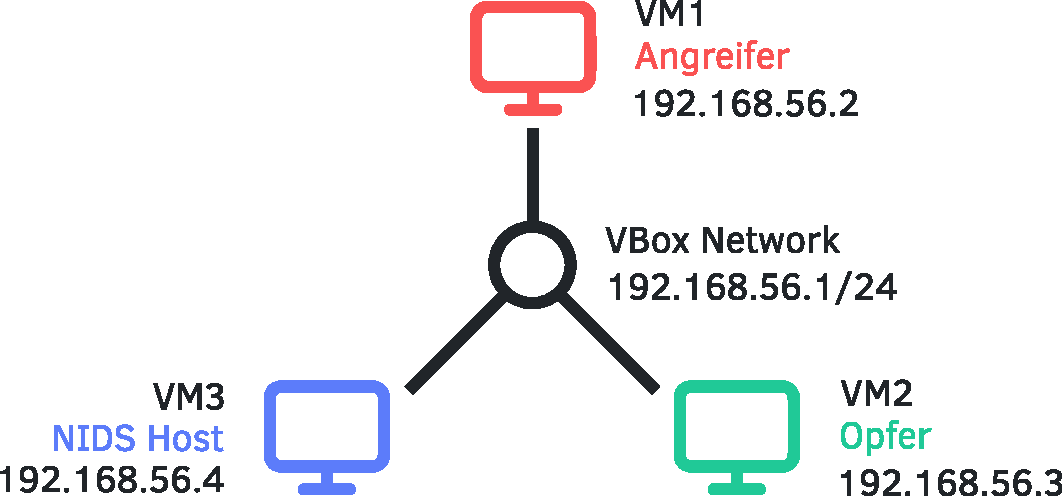
\includegraphics[width=0.6\textwidth]{graphics/intro/network.pdf}
  \caption{Virtuelle Netzwerkstruktur.}\label{fig:network-structure}
\end{figure}

Die drei virtuellen Maschinen befinden sich im gleichen virtuellen Netzwerk. Ein Angreifersystem (Kali Linux) versucht, Hosts im Netzwerk mit unterschiedlichen Methoden anzugreifen. Der NIDS-Host sollte dann mit snort diese Aktivitäten erkennen.\\

Zunächst folgt das Setup der Testumgebung.
